\documentclass{article} % For LaTeX2e
% We will use NIPS submission format
\usepackage{nips13submit_e,times}
% for hyperlinks
\usepackage{hyperref}
\usepackage{url}
% For figures
\usepackage{graphicx}
\usepackage{subfigure}
% math packages
\usepackage{amsmath}
\usepackage{amsfonts}
\usepackage{amsopn}
\usepackage{ifthen}
\usepackage{natbib}

\title{Machine Learning Project I by Group KATHMANDU}

\author{
Jade Copet\\
EPFL \\
\texttt{jade.copet@epfl.com} \\
\And
Merlin Nimier David\\
EPFL \\
\texttt{merlin.nimier-david@epfl.com} \\
\And
Krishna Raj Sapkota\\
EPFL \\
\texttt{krishna.sapkota@epfl.com} \\
}

\nipsfinalcopy

\begin{document}
\maketitle



\begin{abstract}
  In this report, we summarize our findings for the project-I. We analyzed two datasets, regression (D1) and classification (D2).
\end{abstract}



\section{The regression dataset (D1)}

  \subsection{Dataset description}
  Our training data consists of output variable $\mathbf{y}$ and input variables $\mathbf{X}$. We have $N = 1400$ data examples. Each input vector $\mathbf{x}_n$ is of dimensionality $D = 44$. Out of these 44 features, 35 are real-valued while 4 variables are binary and 5 variables are categorical, 4 of them with 4 categories and 1 with 3 categories.

  We also have test data where we do not observe $\mathbf{y}$. We have $N = 600$ test examples. Our goal is to produce predictions for test examples, as well as an approximation of the test error.

  \subsection{Data visualization and cleaning}
  We start by plotting the distribution of the input to obtain Figure \ref{fig:histY}. We notice a gaussian centered around 2500, but also 144 data points above 6500. It represents more than 10\% of our data examples, thus we cannot discard them as outliers: we make the hypothesis that our dataset represents two distinct models.

  Since input variables are not normalized, we center and rescale them before going forward. Plotting each input variable against the output, we notice that feature 35 seems to allow us to separate linearly the two hypothetical models. The categorical variables do not help in an obvious way. To confirm our intuition, we separate points roughly at $X_{35} > 1$ (after normalization) and plot the results in Figure \ref{fig:twoModelsRough}.

  We also investigated the correlation first between output and input variables, and then between features themselves. On one hand, variables 35 and 26 are very correlated with the output with correlation coefficients respectively equal to $0.67$ and $0.43$. The results using only those two variables were quite satisfying but not as good as when using all features. On the other hand, a majority of features are not linearly correlated to the output: for 34 of them the correlation coefficient is less than $0.1$. However this does not suggest removal of all these variables yet as a combination of them may well show higher correlation. Some features are highly correlated to each others: 8 pairs of features have a correlation coefficient higher than $0.5$.\\
  Following from these two observations, we tried to remove one feature of each highly correlated pair which is not significantly correlated to the output. Finally we decided to keep the full input matrix $\mathbf{X}$ for our regression fit since we have not faced any rank-deficiency issue and our results were quite satisfying this way.

  We use the dummy encoding technique for categorical variables (the binary variables do not require dummy encoding). When using the \texttt{dummyvar} function from Matlab, we were cautious to remove one of the resulting columns since it is linearly dependent from the other ones. This gives us a total of 50 input variables and $\mathbf{X}$ still seems well-behaved.

  \begin{figure}[!t]
  \center
  \subfigure[Distribution of output $\mathbf{y}$. There are to many values above 6500 to discard them as outliers.]{
    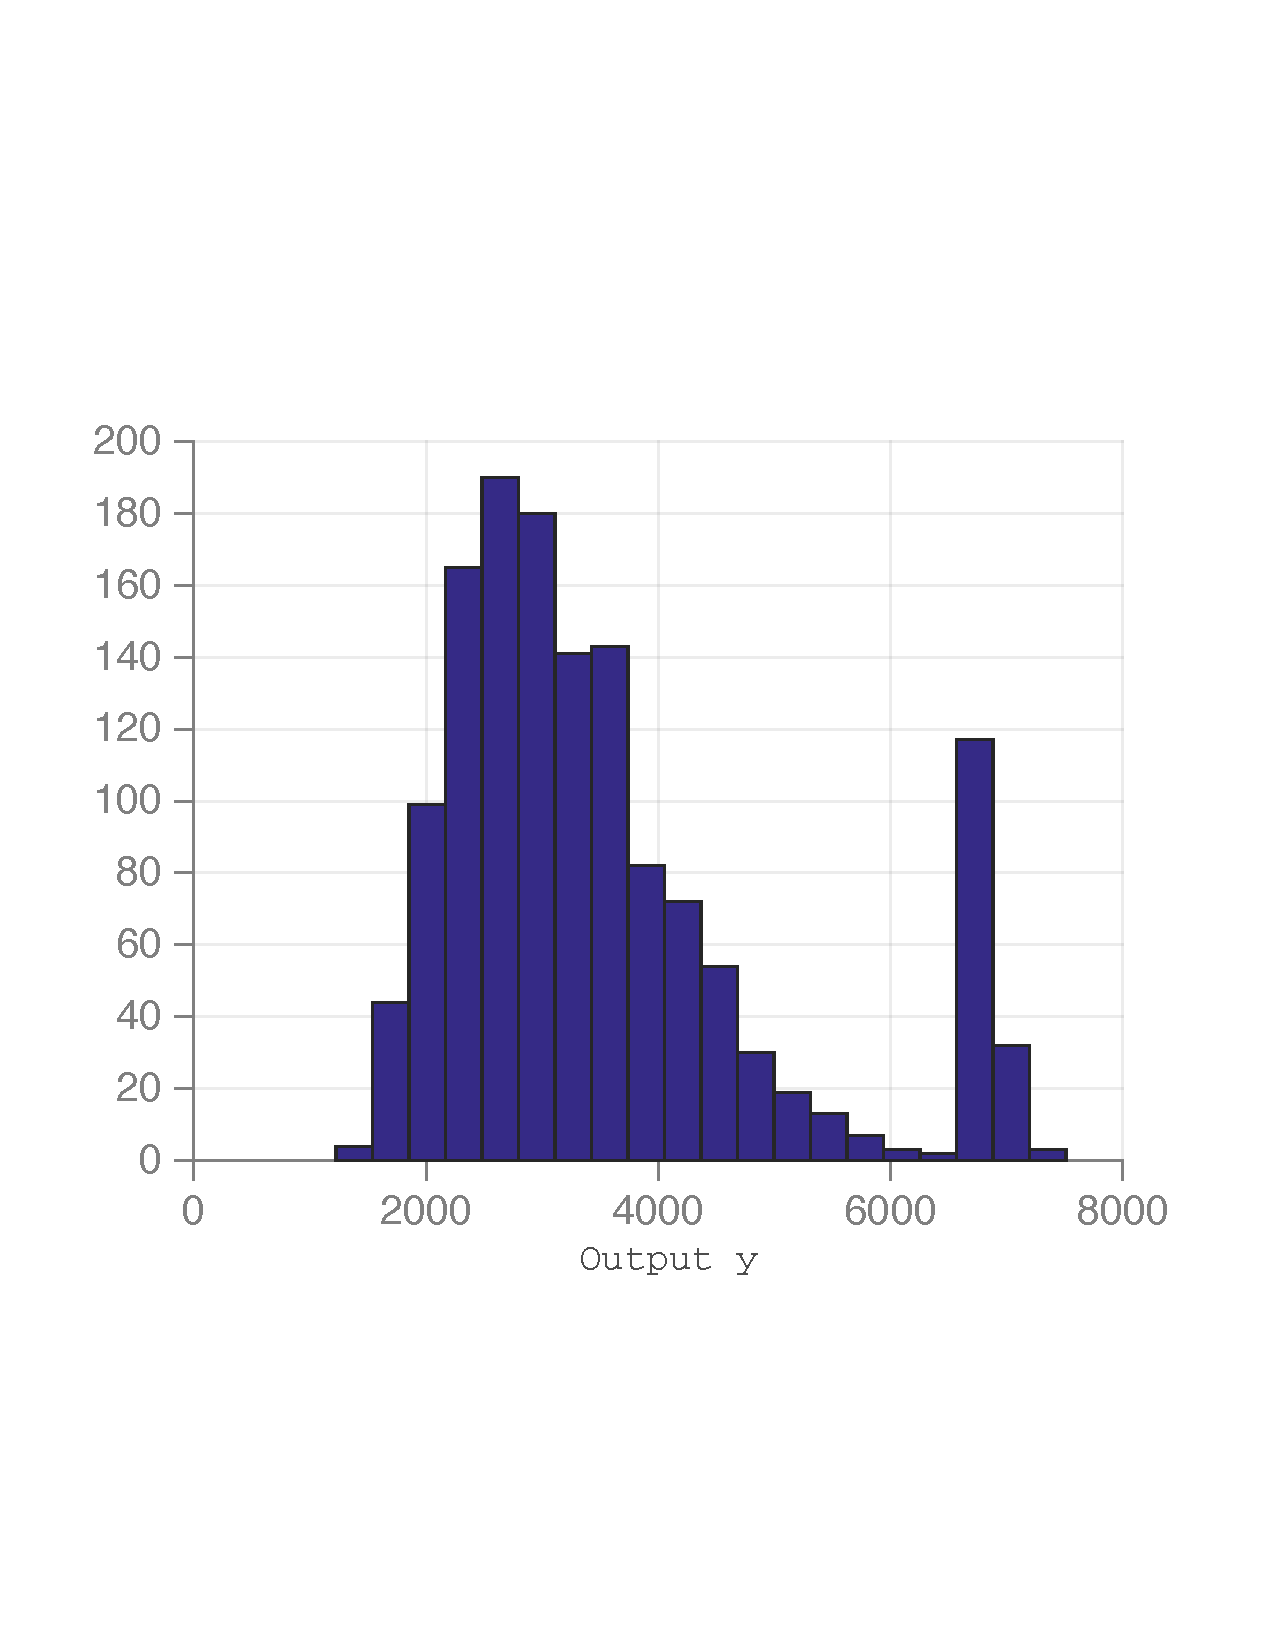
\includegraphics[width=2.5in]{figures/regression/hist-Y.pdf}
    \label{fig:histY}
  }
  \hfill
  \subfigure[$X_{35}$ seems to enable us to linearly separate the two models simply]{
    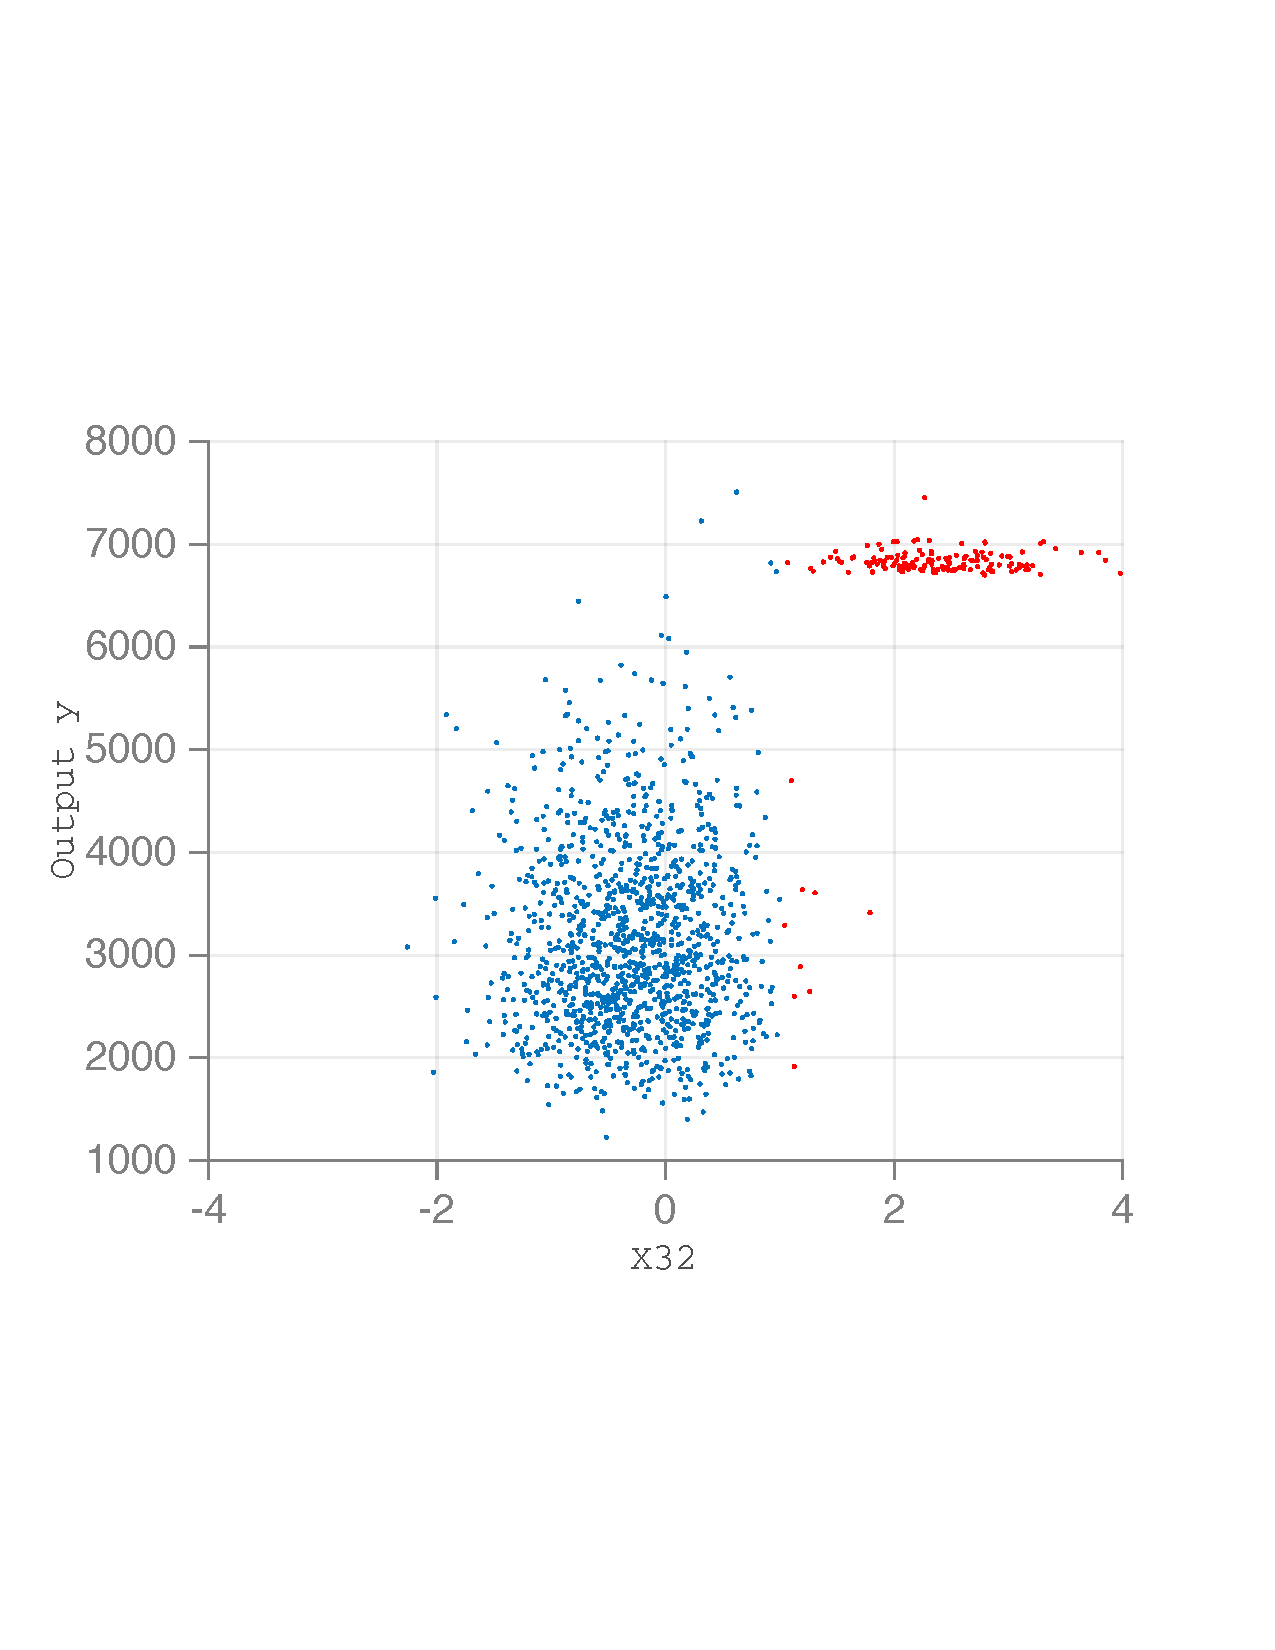
\includegraphics[width=2.5in]{figures/regression/model-separation-X35.pdf}
    \label{fig:twoModelsX35}
  }
  \hfill
  \subfigure[First try at separating the two models using $X_{35} > 1$]{
    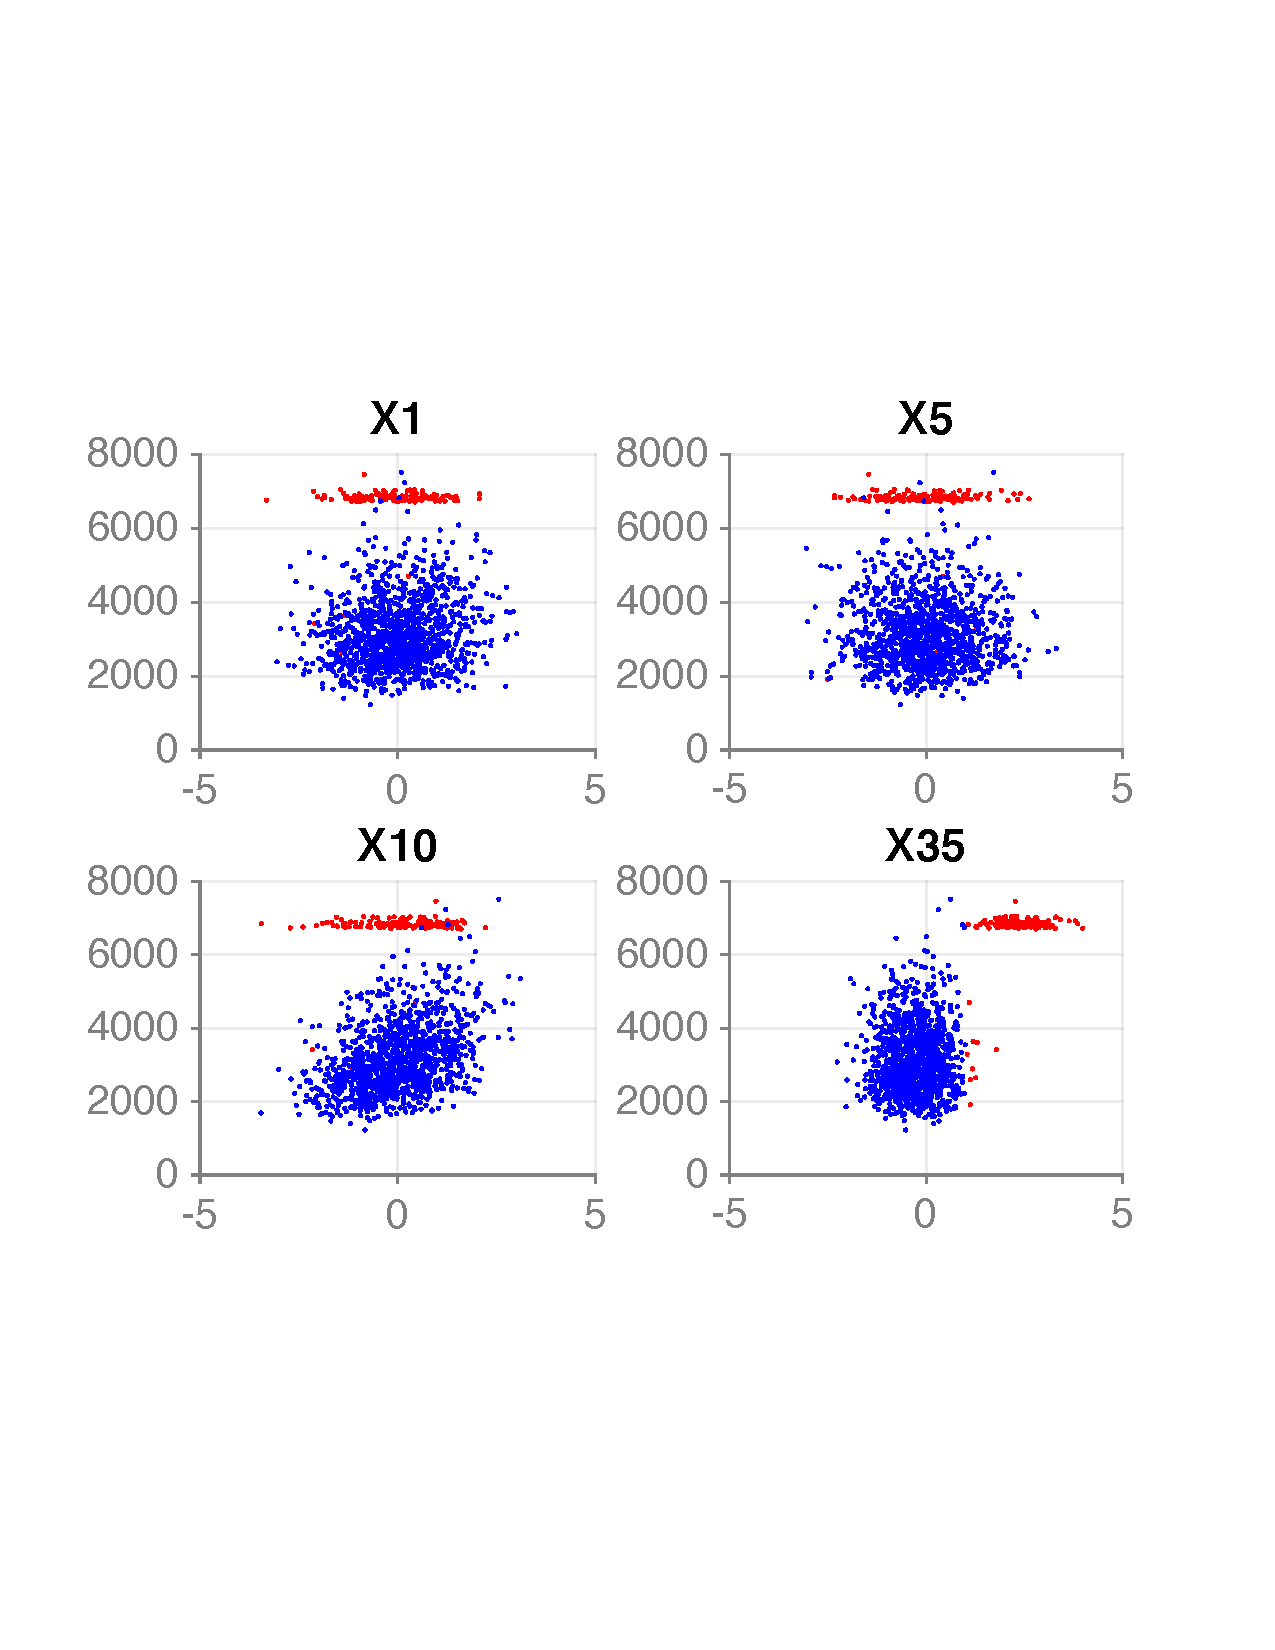
\includegraphics[width=4in]{figures/regression/model-separation-rough.pdf}
    \label{fig:twoModelsRough}
  }
  \caption{}
  \end{figure}

  \subsection{Model separation}
  From our explorative data analysis phase, we emitted the hypothesis that our dataset could be represented by two distinct models. We checked our intuition by learning a single model on the whole dataset, and compared it with a two-model fit learnt over a roughly split dataset. The test error decreased dramatically when using two models. This motivated us to learn a classifier in order to refine the dataset split.

  We chose a threshold on the output value ($y_n > 6200$) and used it to convert $\mathbf{y}$ to a $\{0, 1\}$ label vector. This enabled us to apply logistic regression directly and learn a classifier. We checked the result visually by plotting the two parts of the dataset in different colors.

  The first model, denoted $M_1$, is not trivial. On the other hand, the second model, $M_2$, can be described simply with a (high) constant output value.

  \subsection{Feature transformations}
  In order to describe $M_1$ accurately, we investigated potential feature transformations which would increase the power of expression of our model. We needed to strike a balance between underfitting (purely linear model) and overfitting (high-degree polynomial transformation). To select the degree of polynomial basis expansion, we developed a script which, for each degree:
  \begin{itemize}
    \item Applied polynomial basis expansion up to degree $d$
    \item Created a large number of test / train splits, producing $s$ trials enabling us to validate the stability of our results
    \item For each trial, select the best $\lambda$ penalization parameter using grid search over a logarithmic range of candidate values
  \end{itemize}

  We could then plot the repartition of test and train error over the $s$ trials, allowing us to select the most adapted degree with high confidence about the stability. From Figure \ref{fig:basisExpansionTestError}, a polynomial expansion of degree 4 provides the best expected test error.

  \begin{figure}[h]
    \center
    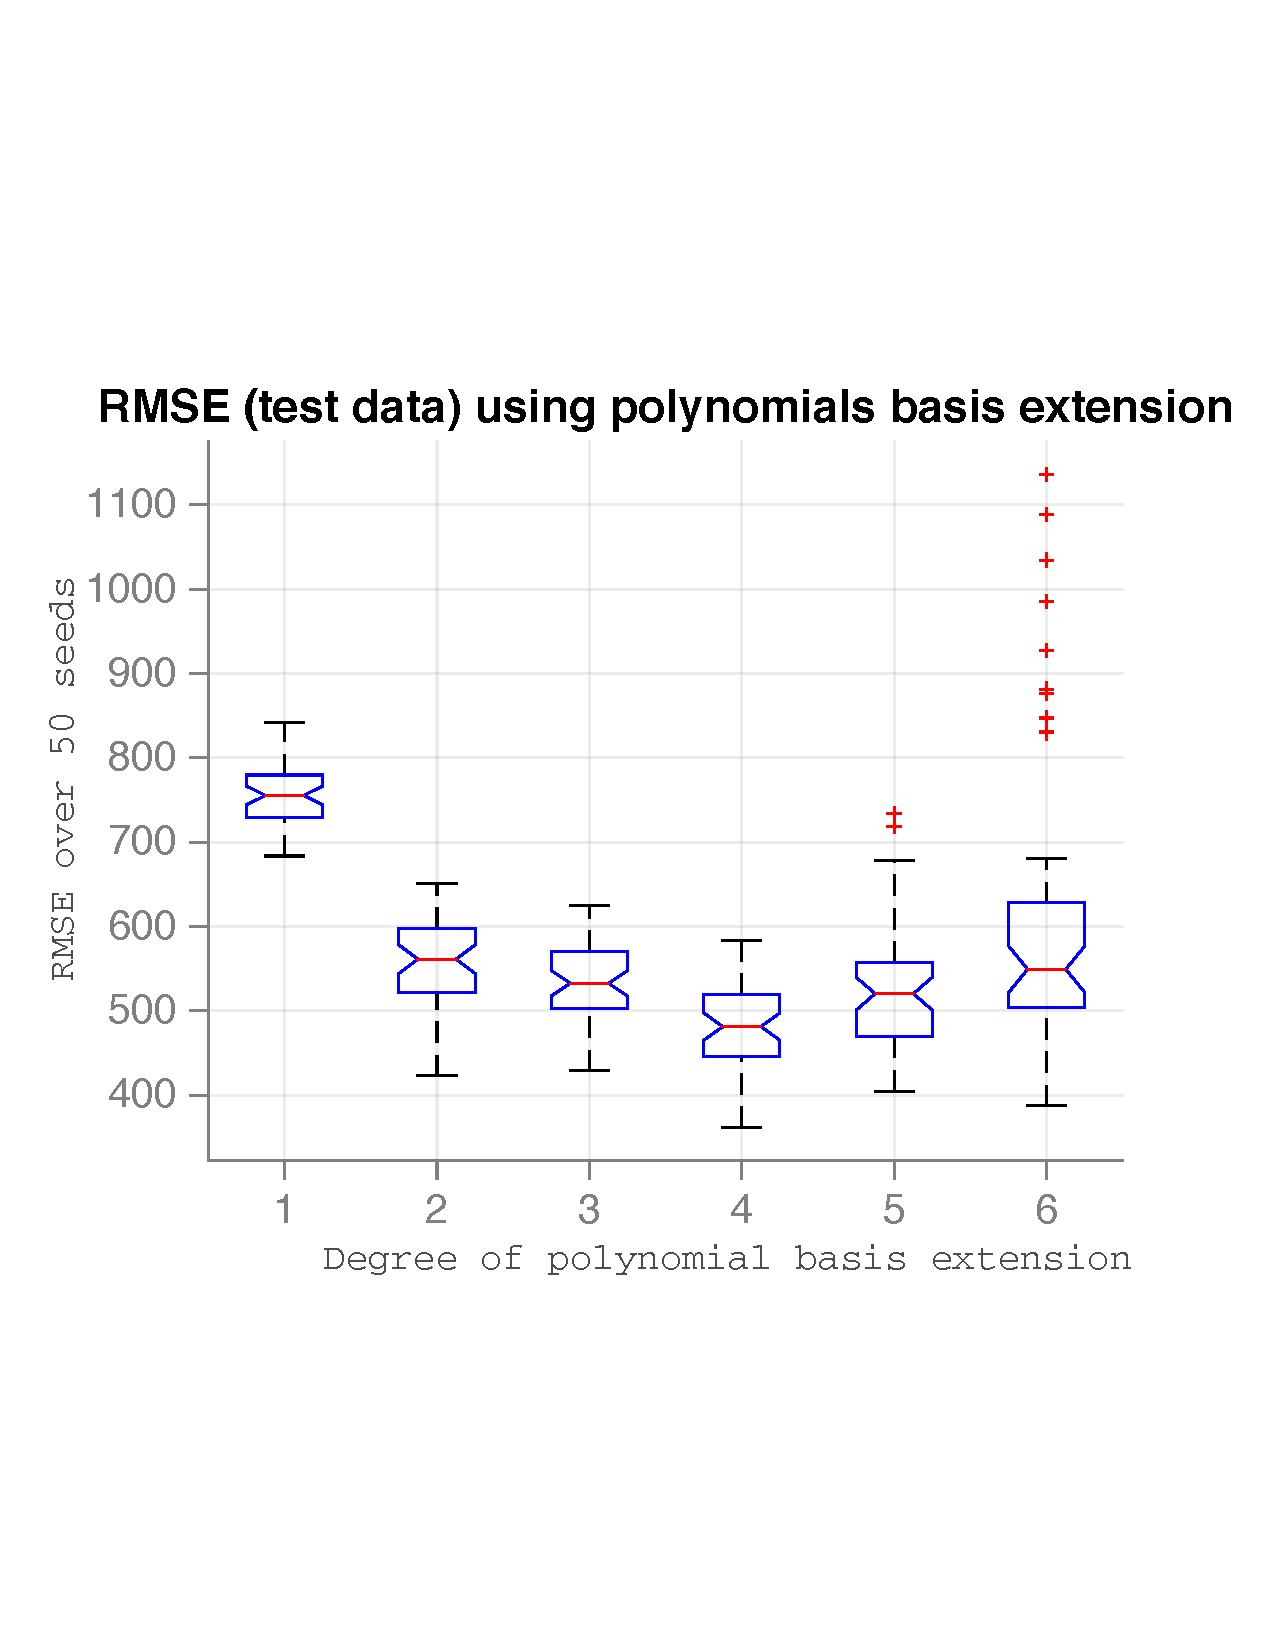
\includegraphics[width=3in]{figures/regression/basis-extension-test-error.pdf}
    \caption{}
    \label{fig:basisExpansionTestError}
  \end{figure}

  We thus chose to apply polynomial expansion to our subset of inputs $X_{M_1}$. We were careful not to transform the binary variables. We obtain dimensionality $D_{M_1} = 156$ and the capacity to overfit, which is why we applied Ridge Regression next to learn our model parameters.

  \subsection{Regression fit and prediction}
  With the necessary data pre-processing done, we were able to easily learn the parameters for our two models:
  \begin{itemize}
    \item $M_1$: model parameter vector $\beta$ was learnt using ridge regression with automatic $\lambda$ selection.
    \item $M_2$: a constant output value equal to the mean of the outputs from the training observations. We were careful to remove obvious outliers.
  \end{itemize}

  We were finaly able to produce our \textbf{hybrid} predictor, which in order:
  \begin{enumerate}
    \item Classified any new input using our learnt classifier.
    \item If the input follows $M_2$, output the learnt constant value.
    \item Otherwise, apply dummy encoding and basis expansion and output the prediction corresponding to model $M_1$ using our learnt predictor $\beta$.
  \end{enumerate}

  We verify the performance of our final predictor by computing its RMSE error and comparing it with simpler predictors over many train / test splits. The average RMSE are summarized in Table \ref{predictorValidation}.

  \begin{table}[h]
    \center
    \begin{tabular}{|r|c|c|}
      \hline
                                              & Train RMSE & Test RMSE \\
      \hline
      Constant output over the whole dataset  & 1.006680   & 0.971525 \\
      \hline
      Least squares over the whole dataset    & 0.512306   & 0.531639 \\
      \hline
      Ridge regression over the whole dataset & 0.523865   & 0.526744 \\
      \hline
      Hybrid predictor                        & 0.320812   & 0.347088 \\
      \hline
    \end{tabular}
    \caption{Validation of our prediction by comparison with simpler models over many train / test splits}
    \label{predictorValidation}
  \end{table}

  Finaly, we produced our predictions for the given \texttt{X\_test} input vector using the hybrid predictor and wrote them to \texttt{regression-output.csv}.

\section{The classification dataset (D2)}
  We applied many of the same techniques to D2.

  \subsection{Dataset description}
  This dataset has $N = 1500$ data examples with dimensionality $D = 32$, as well as $N' = 1500$ test examples. Out of these 32 features, 29 are real-valued and 3 are categorical. Output $\mathbf{y}$ is a binary variable, which implies we are faced with a classification problem. 1052 examples belong to class $C_1$ (for which $y = 0$) and 448 examples belong to $C_2$. Like before, our goal is to produce predictions for test examples, as well as an approximation of the test error.

  \subsection{Data visualization and cleaning}
We performed basic exploratory data analysis on our data. As expected the data is not centered, and therefore we normalize the data. Spotting outliers on a classification dataset is not an easy role, we have assumed that data points are outliers if for any feature they are more than 10 standard deviations away from the median. This gives us a cleaned data set of 1469 examples.

For more convenience in the features manipulation, categorical variables are moved to the last columns of the matrix and we use dummy encoding for each of them. This gives us a total of 46 input variables.

  \subsection{Regression fit}

  \subsection{Feature transformations}

  \subsection{Predictions}



\section{Summary}

\subsubsection*{Acknowledgments}
  We would like to thank Emtiyaz Khan and the teaching assistants for creating this project which was a great opportunity for us to put in practice our knowledge of Machine Learning on a full study-case. We also would like to thank them for their precious advices during the project.\\
  Most ML functions and algorithms were based on code examples provided by the teaching team for the exercise sessions. We developped several exploratory and application scripts to make use of these techniques.
\subsubsection*{References}

\end{document}
